\section{Dashboard - Alles auf einem Blick}
Das Ziel des vorliegenden Kapitel besteht darin einen Überblick über gängige Terminologien und Herangehensweisen in Bezug auf die Erstellung von Dashboards zu geben. 

\subsection{Begriffsdefinition Dashboard} \label{ch:definition_dashboard}
Unter dem Begriff Dashboard wird im Rahmen dieser Arbeit die Begriffsdefinition gemäss Stephen Few verwendet. Stephen beschreibt ein Dashboard als:

\begin{center}
\textbf{``Visual display of the most information needed to achieve one or more objectives which fits entirely on a single computer screen so it can be monitored at a glance.``} ~\citep[S. 34]{information_dashboard_design}  
\end{center}

Ein Dashboard erlaubt es somit der Zielgruppe alle relevanten Informationen auf einen Blick zu erfassen und auf Basis dessen wichtige Entscheidungen zu treffen.

\subsection{Klassifizierung von Dashboards} \label{ch:theory_classification_of_dashboards} \label{ch:classification_of_dashboards}
Es gibt verschiedene Möglichkeiten ein Dashboard zu klassifizieren. Gemäss Few ist eine effektive Methode, welche auch signifikante Unterschiede in Bezug auf das visuelle Design sowie die Ansprüche aufweisst, ist die Klassifizierung gemäss \textbf{Rollen} ~\citep[S. 40]{information_dashboard_design}.

\subsubsection{Strategische Dashboards}
Strategische Dashboards zeichnen sich primär dadurch aus, dass sie die \textbf{zentralen Entscheidungsträger bei ihren strategischen Entscheidungen unterstützen}. Um dies zu erreichen, veranschaulichen strategische Dashboards die notwendigen Informationen auf eine sehr einfache Art und Weise, ohne zu sehr in die Tiefe zu gehen. Eine weitere Eigenschaft von strategischen Dashboards besteht darin, dass \textbf{kein Anspruch auf Echtzeitdaten} besteht, da strategische Entscheidungen Zeit brauchen um korrekt getroffen zu werden. Es reicht daher, wenn die Daten täglich, wöchentlich oder monatlich aktualisiert werden. Strategische Dashboards bieten im Gegensatz zu analytischen Dashboards \textbf{keine direkten Interaktionsmöglichkeiten} mit den Visualisierung, wenn es um die Auswertung und Analyse der Daten geht und repräsentieren eine statische Momentaufnahme ~\citep[S. 41]{information_dashboard_design}.

\subsubsection{Analytische Dashboards}
Gleich wie strategische Dashboards haben analytische Dashboards in der Regel \textbf{keinen Anspruch auf Echtzeitdaten}. Jedoch erlauben analytische Dashboards die \textbf{Interaktion mit den Daten} zum Beispiel mit Hilfe von Filtereinstellungen und Drill-Down Funktionalitäten ~\citep[S. 41]{information_dashboard_design}. Eine Drill-Down Funktionalität erlaubt es hierbei von einer Übersichtsseite in eine spezifischere Detailseite des Dashboards zu wechseln. Die Daten aus der Übersichtsseite werden ``aufgebohrt`` und im Rahmen einer Detailseite mit weiteren Kontextbezogenen Informationen dargestellt. Ein analytisches Dashboard erlaubt es somit die Datengrundlage genauer zu analyiseren. Es ist daher von zentraler Bedeutung, dass ein analytisches Dashboard logisch aufgebaut ist um eine zielführende Datenanalyse zu unterstützen.

\subsubsection{Operative Dashboards}
Das Hauptaugenmerk liegt bei einem operativen Dashboard auf seiner dynamischen Natur. Anders als strategische und analytische Dashboards ist ein operatives Dashboard stark auf \textbf{Echtzeitdaten und dynamische Interaktionen} angewiesen. So muss das operative Dashboard zum Beispiel im Falle eines schwerwiegenden Fehlers die Zielgruppe unmittelbar benachrichtigen. Wie bei einem strategischen Dashboard müssen die Visualisierungen verständlich sein. Der \textbf{Informationsgehalt} bei einem operativen Dashboard ist jedoch \textbf{sehr spezifisch} und stark auf den Kontext fokussiert ~\citep[S. 42]{information_dashboard_design}.

\subsection{Auswahl der Daten}
Ein zentrales Kriterium bei der Erstellung eines Dashboards ist die Auswahl der korrekten Daten. In Bezug auf die Daten unterscheidet man zwischen \textbf{quantitativen} sowie \textbf{nicht quantitativen} Daten.

\subsubsection{Quantitative Daten}
Gemäss Few werden auf Dashboards primär \textbf{quantitative Daten} dargestellt ~\citep[S. 43]{information_dashboard_design}. Unter quantitative Daten sind hierbei Daten zu verstehen, welche einen Überblick über den aktuellen Zustand erlauben. Eine Möglichkeit um quantitative Daten zu ermitteln besteht darin, Kategorien zu bilden. Die Studie von Zhang hat bei der Erstellung des Codebooks automatisch bereits ein Kategoriensystem aufgrund der Nachrichtenkategorie geschaffen (siehe Kapitel \ref{ch:landscape_of_covid_data_visualization}). Somit ist eine mögliche Kategorie zum Beispiel ``Ìnforming of the severity``, die entsprechenden quantitativen Daten zur Kategorie wären zum Beispiel Corona Ansteckungszahlen (siehe Abbildung \ref{fig:zhang_codebook_intended_message}). 

\subsubsection{Nicht Quantitative Daten}
In Bezug auf Corona spielen nebst den quantitativen Daten wie Ansteckungszahlen etc. ebenfalls nicht quantitative Daten eine grosse Rolle. Mögliche Beispiele von nicht quantitativen Daten, welche auf einem Corona Dashboard durchaus Sinn ergeben sind zum Beispiel Corona Schutzmassnahmen in Form von Infografiken wie sie das \gls{bag} angefertigt hat (siehe Abbildung \ref{fig:bag_infographic}).


 \begin{figure}[h]
    
\includegraphics[width=12cm]{images/bag_covid_infographic.png}
    \centering
    \caption{Erstellte Infografik in Bezug auf Schutzmassnahmen bezüglich Corona ~\citep[S. 1]{bag_covid_infographic}}
    \label{fig:bag_infographic}
\end{figure}
 

\subsection{Allgemeine Fehlerquellen beim Dashboard Design}
Ein informatives und leicht verständliches Dashboard zu gestalten ist keine einfache Aufgabe, vorallem dann nicht wenn Informationen innerhalb eines Bildschirms ihren Platz finden müssen. Few identifiziert in diesem Zusammenhang 13 allgemeine Fehlerquellen in Bezug auf Dashboard Design ~\citep[S. 49]{information_dashboard_design}. Nachfolgend wird auf die relevantesten Fehlerquellen genauer eingegangen.

\subsubsection{Die Grenzen des Sichtbaren überschreiten}
Gemäss der Dashboard Definition (siehe Kapitel \ref{ch:definition_dashboard}) sollten sämtliche Informationen auf einem Bildschirm sichtbar sein. Ein Fehler in diesem Zusammenhang, welcher gemäss Few gemacht wird, ist das \textbf{Platzieren von Visualisierungen ausserhalb des sichtbaren Bereiches}, sodass es für den Nutzer notwendig wird zu scrollen. Nutzer nehmen Dinge im aktiven Sichtfeld viel prägnanter wahr, als solche welche ausserhalb des Sichtfeldes liegen. Few argumentiert hierzu, dass Dinge welche \textbf{ausserhalb des sichtbaren Bereichs liegen automatisch weniger wichtig sind} und daher nur selten die Beachtung des Nutzers finden ~\citep[S. 50-53]{information_dashboard_design}.

\subsubsection{Informationen mit zu hohem Detaillierungsgrad}
Eine weitere Fehlerquelle ist die Darstellung von Daten mit einem zu hohen Detaillierungsgrad. Ein Beispiel hierzu wäre die Berechung von Schulnoten. So könnte die Note im Fach Mathematik zum Beispiel mit 5.3275 dargestellt werden, wobei es völlig ausreicht, diese mit 5.3 zu beziffern. \textbf{Die Genauigkeit der Information und somit der Detaillierungsgrad sind jedoch sehr stark vom Kontext abhängig} und muss mit Bedacht gewählt werden, um den Nutzer nicht zu überfordern ~\citep[S. 55-56]{information_dashboard_design}.

\subsubsection{Einsatz von nicht geeigneten Datenvisualisierungen}
Um die Daten verständlich zu veranschaulichen ist die Wahl der korrekten Datenvisualisierung von hoher Bedeutung. Ein Beispiel hierzu ist die Verwendung von Kuchendiagrammen anstelle eines besser geeigneten Balkendiagramms. Kuchendiagramme werden dazu verwendet, wenn es um die Visualisierung von Daten als Teil des Ganzen geht ~\citep[S. 59]{information_dashboard_design}. Jedoch muss bei einem Kuchendiagramm jedes Teilstück entsprechend beschriftet und mit einer Prozentangabe versehen werden, dies wird im Falle von vielen Teilstücken unübersichtlich. Zudem ist es für den Nutzer nicht leicht, kleine Unterschiede in ähnlichen Teilstücken (mit fast gleichem Prozentwert) zu erkennen. Hier funktionieren Balkendiagramme sehr viel besser (siehe Abbildung \ref{fig:pie_vs_bar_chart}).

\begin{figure}[h]
    \includegraphics[width=12cm]{images/pie-vs-bar-chart.png}
    \centering
    \caption{Falsche Verwendung von Datenvisualisierungen ~\citep{pie_vs_bar_chart}}
    \label{fig:pie_vs_bar_chart}
\end{figure}


\subsubsection{Falsche Verwendung von Farben} \label{ch:introduction_colors}
Farben sind ein wichtiges Instrument um die Aufmerksamkeit des Nutzers zu wecken. Jedoch können Sie bei falscher Verwendung die Wichtigkeit der Daten verschleiern. Gemäss Few sollten Farben mit Bedacht gewählt und auf einem fundierten Grundverständniss über die Funktionsweise von Farben erfolgen. Wichtige Daten sollten entsprechend mit warmen Farben, welche unsere Aufmerksamkeit wecken, hervorgehoben werden (siehe Abbildung \ref{fig:standard_and_emphasis_colors}). Bei der Auswahl von Farben sollten jedoch auch farbenblinde Nutzer berücksichtigt werden. Gemäss Few sind rund 10\% der Männer sowie 1\% der Frauen farbenblind. Um diesen Personenkreis zu berücksichtigen, können Farbabstufungen verwendet werden ~\citep[S. 75 + 154]{information_dashboard_design}.

\begin{figure}[h]
    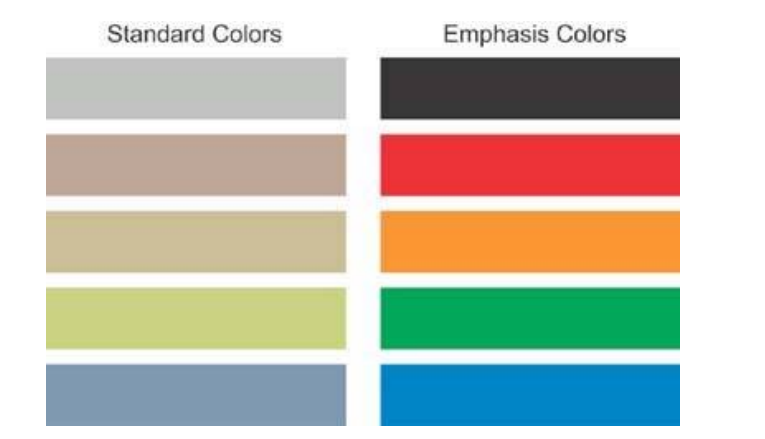
\includegraphics[width=12cm]{images/standard_and_emphasis_colors.png}
    \centering
    \caption{Standard und Betonungsfarben ~\citep[S. 89]{information_dashboard_design}}
    \label{fig:standard_and_emphasis_colors}
\end{figure}

\subsection{Die Gestaltprinzipien}
Durch das Einhalten etablierten Design Prinzipien wie zum Beispiel den Gestaltprinzipien von Wertheimer kann die visuelle als auch informative Qualität des Dashboards gesteigert werden. Die Gestaltprinzipien, welche sich mit der menschlichen Warhnehmung von Objekten befassen, wurden zwischen 1910 und 1920 vom deutschen Psychologen May Wertheimer entwickelt ~\citep{gestalt_prinzipien}. Wird die Wahrnehmung von Objekten verstanden, so lassen sich wichtige Daten und Informationen effektiver hervorheben und unterstützen dabei effektivere Datenvisualisierungen und Dashboards zu gestalten. Nachfolgend wird auf die wichtigsten Gestaltprinzipien eingegangen.

\clearpage
\subsubsection{Das Gesetz der Nähe}
Das Gesetz der Nähe besagt, dass Menschen Objekte, welche sich in der Nähe voneinander befinden, der gleichen Gruppe zuordnet (siehe Abbildung \ref{fig:principle_of_proximity}). Das Gesetz der Nähe kann dazu verwendet werden um Daten welche zusammen gehören visuell besser hervorzuheben ~\citep[S. 90]{information_dashboard_design}.

\begin{figure}[h]
    
\includegraphics[width=12cm]{images/principle_of_proximity.png}
    \centering
    \caption{Das Gesetz der Nähe ~\citep[S. 90]{information_dashboard_design}}
    \label{fig:principle_of_proximity}
\end{figure}


\subsubsection{Das Gesetz der Ähnlichkeit}
Der Mensch hat die Tendenz Objekte mit ähnlicher Farbe, Grösse oder Orientierung der gleichen Gruppe zuzuordnen. Wenn die gleichen Daten in unterschiedlichen Arten dargestellt werden (Corona Fallzahlen als Linien- und Balkendiagramm), kann alleine über die Verwendung der gleichen Farbe eine Verknüpfung hergestellt werden ~\citep[S. 91-92]{information_dashboard_design}.

\clearpage
\subsubsection{Das Gesetz der gemeinsamen Region}
Das Gesetz der gemeinsamen Region besagt, dass Menschen Objekte, welche mit einer visuellen Abgrenzung (beispielsweise eines Rahmens) versehen sind, der gleichen Gruppe zuordnen ~\citep[S. 92]{information_dashboard_design}. Die Willkommensseite von Google Data Studio wendet dieses Prinzip ebenfalls an und nutzt Rahmen um die einzelnen Elemente visuell voneinander abzugrenzen (siehe Abbildung \ref{fig:principle_of_enclosure}). 

\begin{figure}[h]
    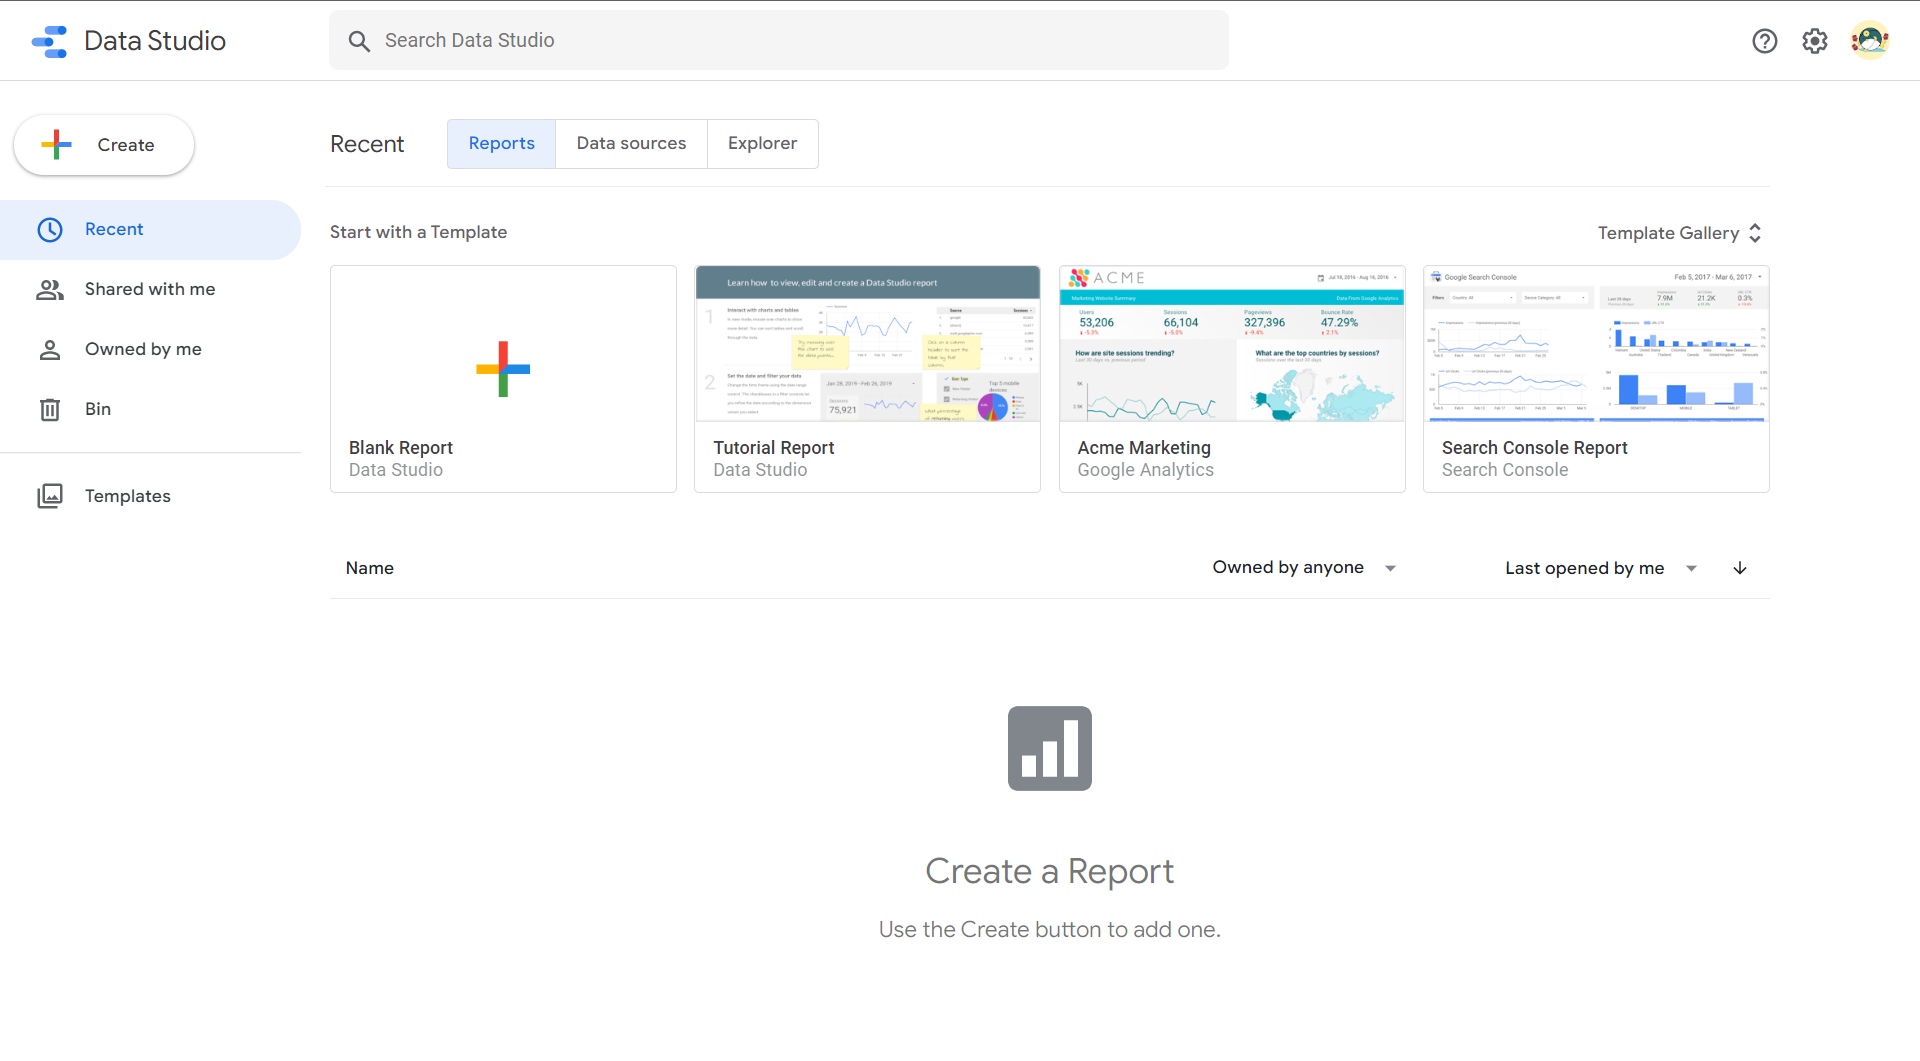
\includegraphics[width=12cm]{images/principle_of_enclosure.png}
    \centering
    \caption{Das Gesetz der gemeinsamen Region ~\citep{principle_of_enclosure_google_data_studio}}
    \label{fig:principle_of_enclosure}
\end{figure}

\subsection{Die 8 Goldenen Regeln von Ben Shneiderman}
Ben Shneiderman entwickelte 8 Regeln, welche beachtet werden sollten, wenn es um die Entwicklung von User Interface Design geht ~\citep{shneiderman_golden_rules}. Diese Regeln sollten ebenfalls für die Erstellung eines Dashboards berücksichtigt werden.

\subsubsection{Einhaltung der Konsistenz}
Die Einhaltung der Konsistenz kann gemäss Shneiderman durch die Verwendung einheitlicher Layouts, Farbgebungen sowie Schriftarten erreicht werden. Ein weiterer wichtiger Aspekt, vorallem im Zusammenhang mit Daten, ist die Einhaltung einer einheitlichen Terminologie der Begrifflichkeiten ~\citep{shneiderman_golden_rules}.

\subsubsection{Universelle Verwendbarkeit}
Je nach Wissensstand und Fähigkeiten einer bestimmten Nutzergruppe müssen unterschiedliche Funktionalitäten und Detaillierungsebenen zur Verfügung gestellt werden. Für einen unerfahrenen Nutzer sind beispielsweise Hilfestellungen mittels Tooltipps notwendig, wohingegen ein erfahrener Nutzer Shortcuts bevorzugt ~\citep{shneiderman_golden_rules}.

\subsubsection{Informatives Feedback}
Für jede Aktion, die ein Benutzer durchführt, sollte entsprechend informatives Feedback zur Verfügung gestellt werden. Bei häufig durchgeführten Aktionen kann das Feedback kurz und prägnant sein, wohingegen bei seltenen Aktionen ein ausführlicheres Feedback notwendig ist ~\citep{shneiderman_golden_rules}.

\subsubsection{Entwicklung von abschliessenden Dialogen}
Aktionen welche der Nutzer durchführen kann, sollten einem logischen Ablauf folgen. Dies kann zum Beispiel durch eine Gruppierung der Aktionen erfolgen. Shneiderman bringt hierzu als Veranschaulichungsbeispiel den Besuch von E-Commerce Seiten (beispielsweise digitec.ch) auf. Beim Besuchen von digitec.ch sucht sich der Nutzer zuerst ein Produkt aus. Anschliessend legt er das Produkt in den Warenkorb, gibt Versandadresse an und bestätigt zum Schluss den Kauf ~\citep{shneiderman_golden_rules}. Somit kann beispielsweise der Ablauf bei E-Commerce Seiten in die Kategorien ``Produktauswahl``, ``Angaben der Lieferoptionen`` sowie ``Abschluss`` unterteilt werden.

\subsubsection{Vermeidung von Fehlern}
Das User Interface sollte so konzipiert werden, dass möglichst wenig Fehlerpotenzial vorhanden ist. Dies kann bereits mithilfe von einfachen Formularvalidierungen (beispielsweise Validierung von E-Mail Adressen) erreicht werden. Tritt jedoch ein Fehler auf, so muss dem Nutzer eine einfache Möglichkeit zur Verfügung stehen, wieder in einen Normalzustand zurückzukehren ~\citep{shneiderman_golden_rules}.

\subsubsection{Möglichkeit, Aktionen rückgängig zu machen}
Der Nutzer sollte die Möglichkeit besitzen, von ihm durchgeführte Aktionen wieder rückgängig machen zu können. Gemäss Shneiderman können hierbei einzelne Aktionen oder mehrere Aktionen rückgängig gemacht werden ~\citep{shneiderman_golden_rules}.

\subsubsection{Kontrolle liegt in den Händen der Nutzer}
Die Kontrolle über das User Interface sollte zu jedem Zeitpunkt in den Händen der Nutzer liegen. Verhaltensweisen des User Interfaces, welche zur erneuten Eingaben von Daten (beispielsweise Formulardaten) führen sind zu vermeiden ~\citep{shneiderman_golden_rules}.

\clearpage
\subsubsection{Belastungsreduktion des Kurzzeitgedächnis}
Das Kurzzeitgedächnis kann nur eine bestimmte Menge von Informationen speichern. Sämtliche notwendigen Informationen sollten daher auf einen Blick verfügbar sein. Ansichten, welche das Merken von ``alten Informationen`` verlangen um vollumfänglich verständlich zu sein, sollten vermieden werden ~\citep{shneiderman_golden_rules}.

\subsection{Software Lösungen für die Gestaltung von Dashboards}
Gemäss Stephen Few gibt es verschiedene Arten Dashboards zu implementieren, die korrekte Lösung hängt hierbei jedoch vom Anwendungsfall ab ~\citep[S. 34]{information_dashboard_design}. Als Grundlage für die Auswahl der nachfolgenden Technologien dient die Studie von Barbazza (siehe Abbildung \ref{fig:software_for_creating_dashboards}). Gemäss Barbazza wurden die meisten Dashboards mithilfe von \textbf{kommerziellen Lösungen} (58\%) sowie \textbf{In-House Lösungen} (42\%) entwickelt ~\cite[S. 9]{barbazza}. Nachfolgend wird auf die wichtigsten kommerziellen Lösungen für die Gestaltung von Dashboards eingegangen. In Bezug auf In-House Lösungen wird der Fokus explizit auf \textbf{frei verfügbare Web-Technologien} gelegt.

\begin{figure}[h]
    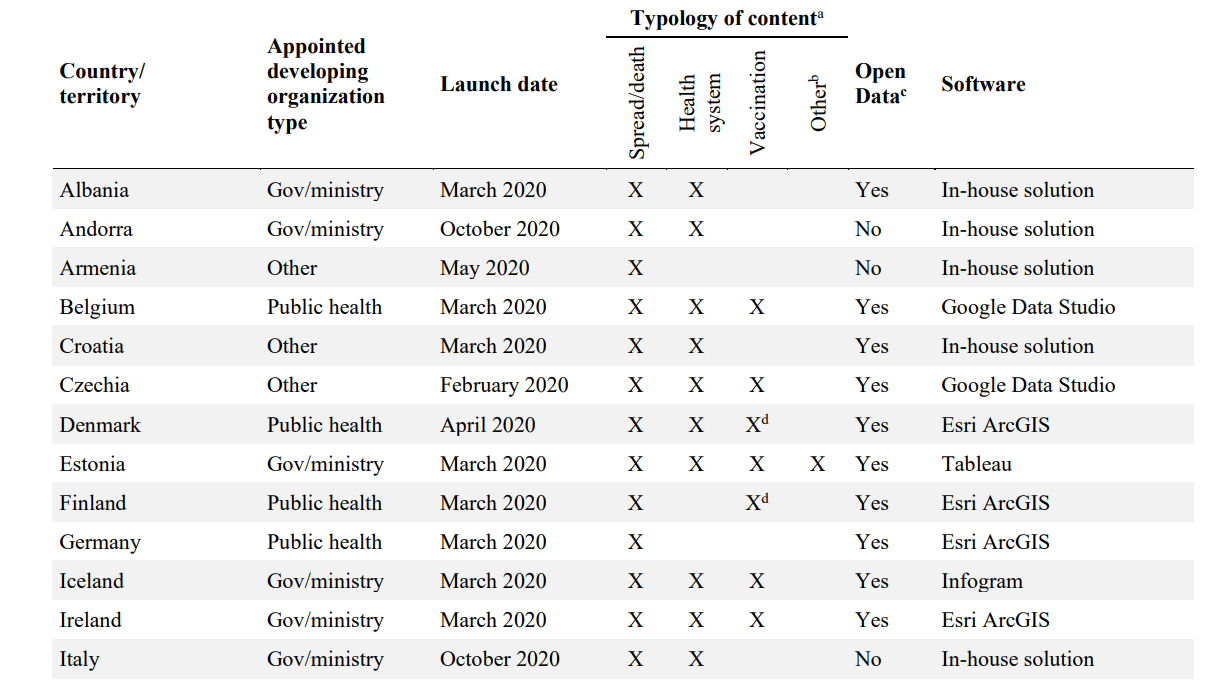
\includegraphics[width=12cm]{images/software_for_creating_dashboards.png}
    \centering
    \caption{Auszug aus der Softwarelandschaft zur Erstellung von Corona Dashboards gemäss Barbazza ~\citep[S. 11]{barbazza}}
    \label{fig:software_for_creating_dashboards}
\end{figure}

\clearpage
\subsubsection{Kommerzielle Lösungen} \label{ch:theory_commercial_solutions}

\noindent
\textbf{Esri ArcGIS}
\newline
\indent
ArcGIS ist spezialisiert auf die Darstellung von Daten, welche mit Ortsangaben verbunden sind, was sich auch als Teil des Namens mit dem Suffix \gls{gis} wiederspiegelt. Die \textit{Spezialisierung auf ortsabhängige Daten} machen ArcGIS eine gute Wahl, für die Erstellung von Corona Dashboards. Dies zeigt auch die Studie von Barbazza, gemäss welcher rund 33\% der Dashboards mit Esri ArcGIS entwickelt ~\citep[S. 9]{barbazza} wurden.  Das wichtigste Produkt im Kontext dieser Arbeit ist hierbei das Dashboard Modul von ArcGIS (siehe Abbildung \ref{fig:arcgis_dashboard_module}). Mithilfe dieser Software ist es möglich Dashboards für verschiedene Rollen zu erstellen (siehe Kapitel \ref{ch:classification_of_dashboards}).

\begin{figure}[h]
    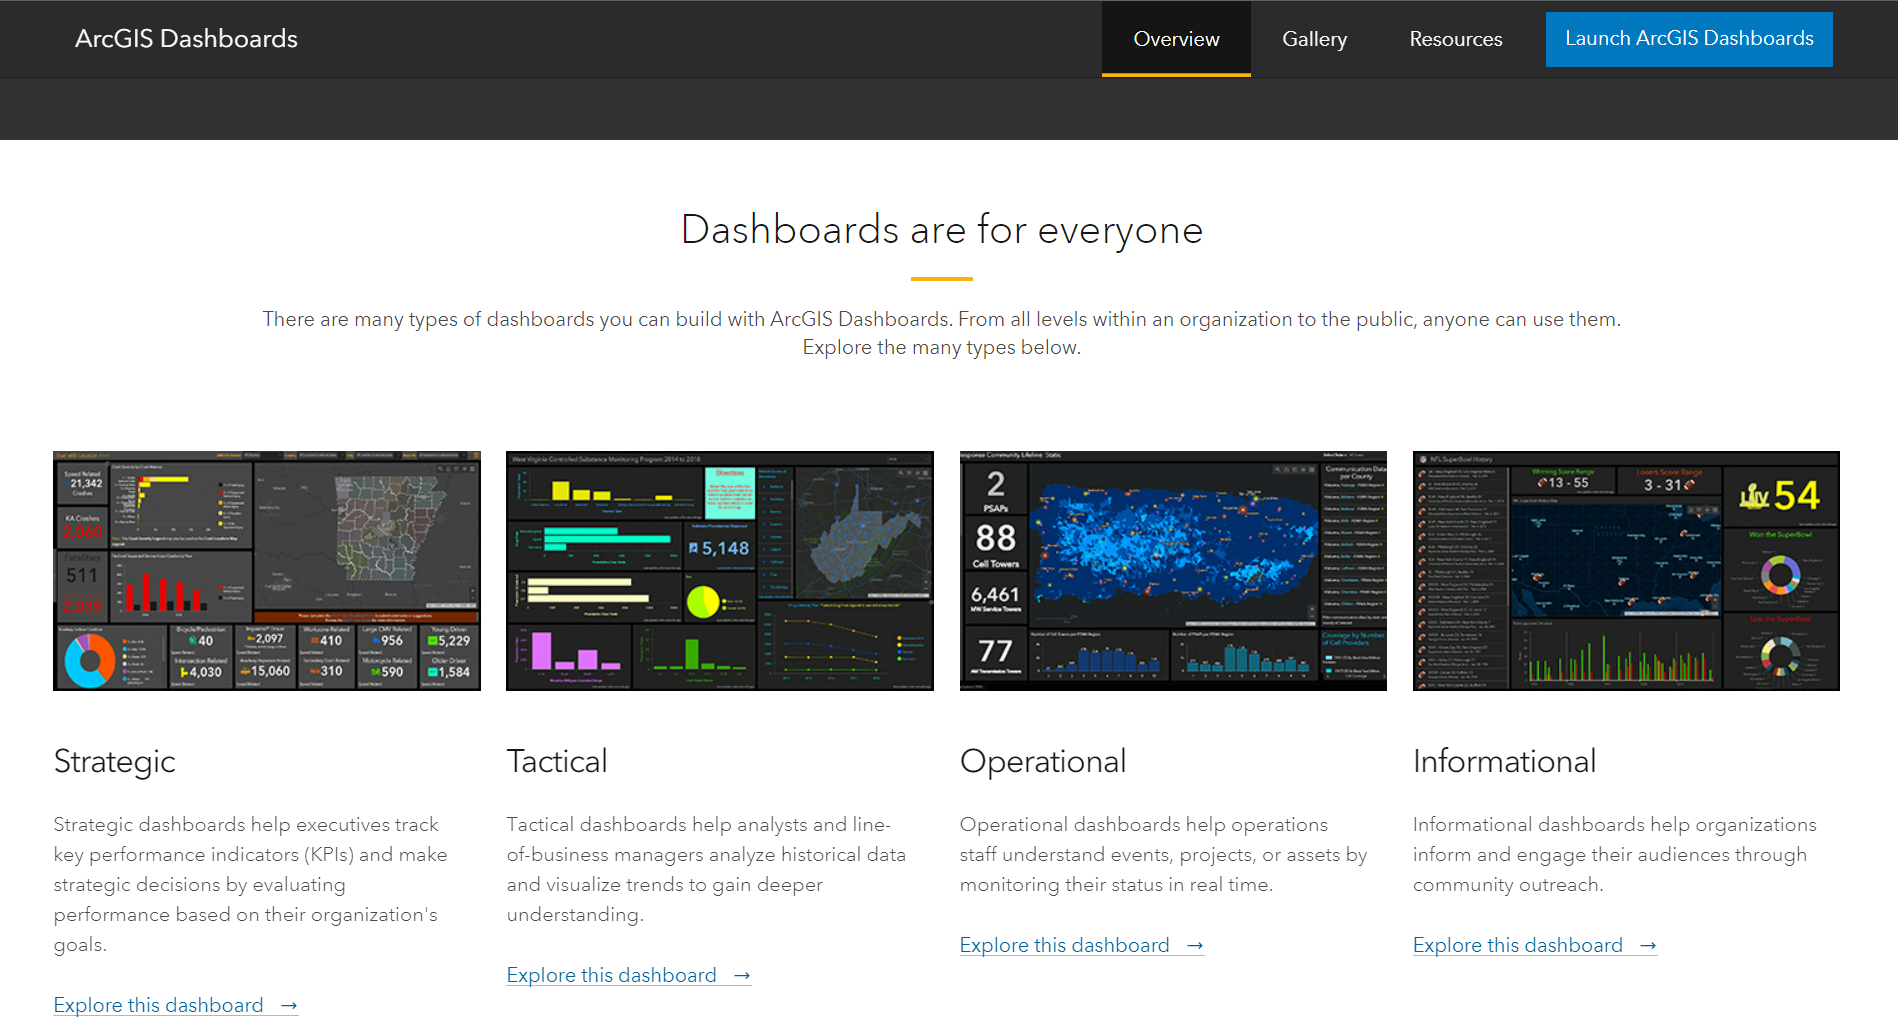
\includegraphics[width=12cm]{images/arcgis_dashboard_solution.png}
    \centering
    \caption{Dashboard Modul von ArcGIS ~\citep{arcgis_dashboard_solution}}
    \label{fig:arcgis_dashboard_module}
\end{figure}

Ein bekanntes Beispiel für ein entwickeltes Corona Dashboard ist hierbei das Dashboard der Hopkins Universität (siehe Abbildung \ref{fig:arcgis_hopkins_dashboard}). Ein Nachteil der ArcGIS Software ist die \textit{eingeschränkte Anpassbarkeit} der Dashboard Layouts sowie der \textit{hohe Preis} ~\citep{arcgis_comparison}.


\begin{figure}[h]
    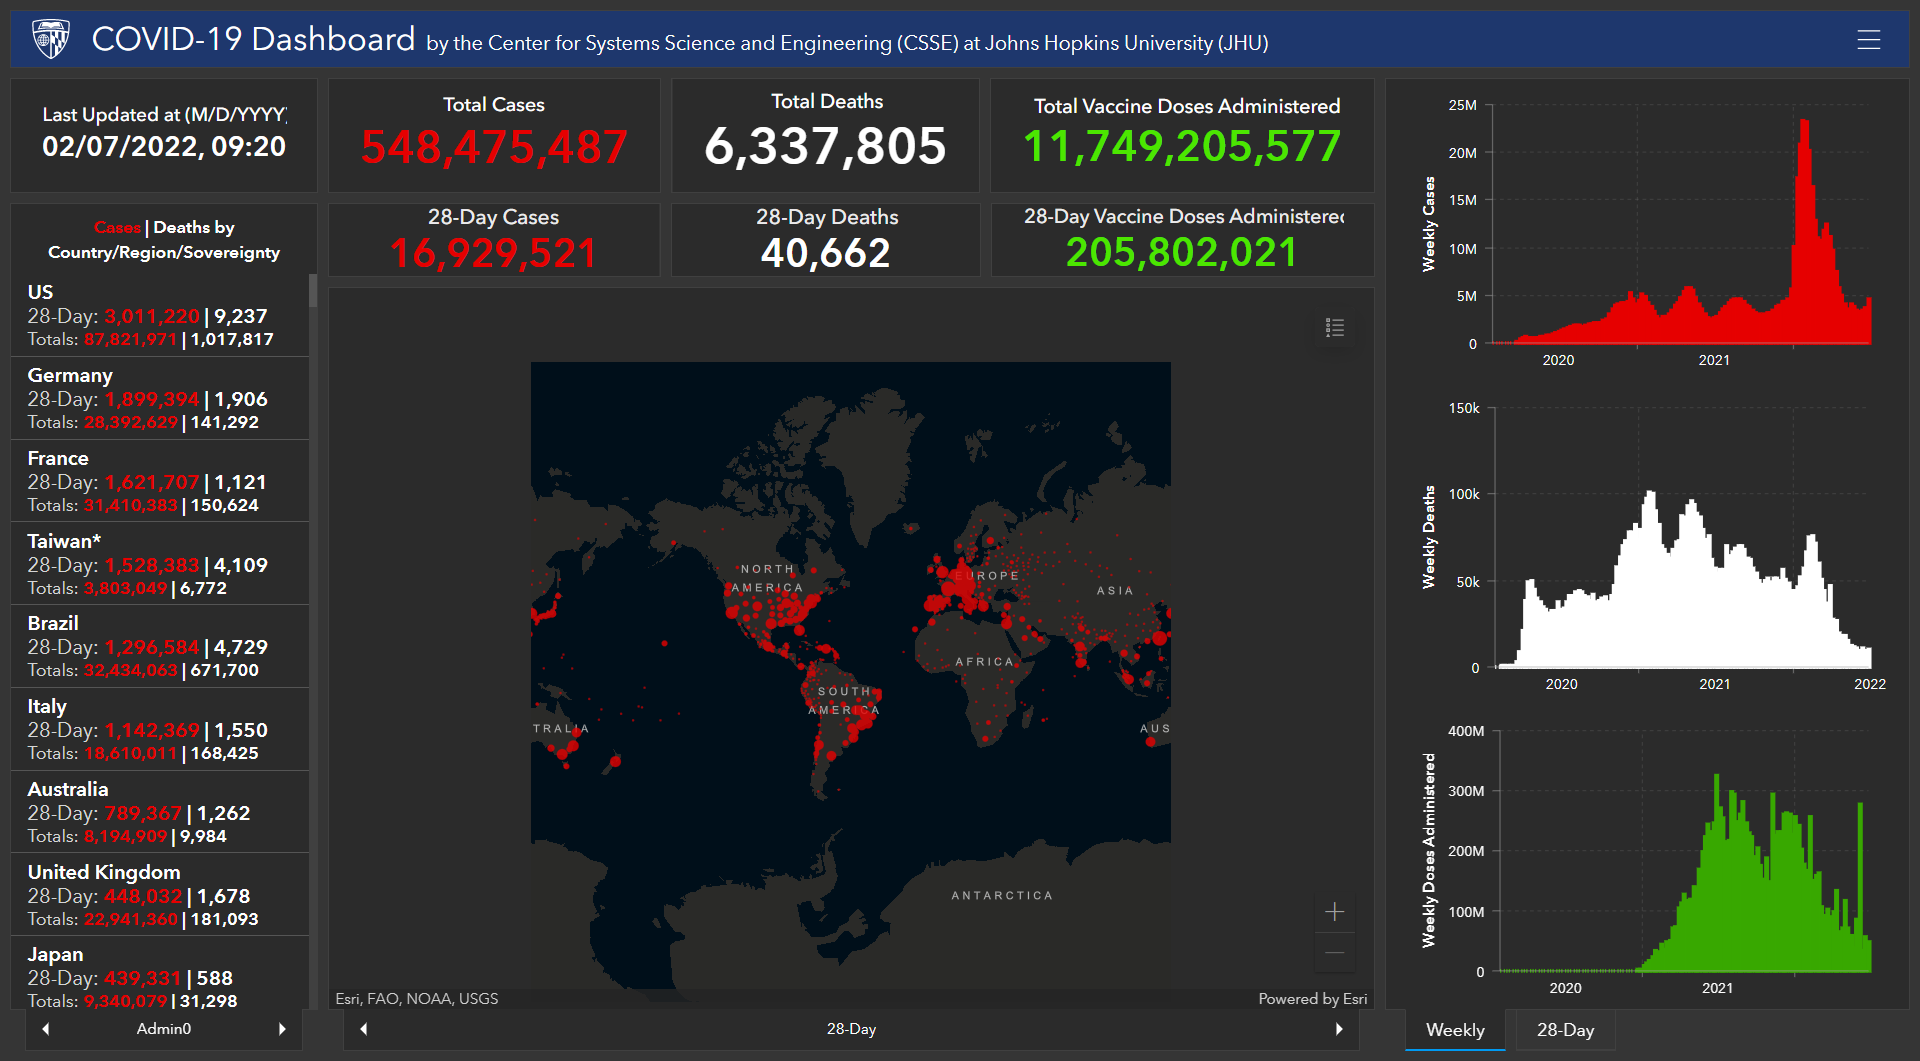
\includegraphics[width=10cm]{images/arcgis_hopkins_dashboard.png}
    \centering
    \caption{Hopkins Corona Dashboard welches mithilfe von ArcGIS entwickelt wurde ~\citep{arcgis_hopkins_dashboard}}
    \label{fig:arcgis_hopkins_dashboard}
\end{figure}


\clearpage
\noindent
\textbf{Google Data Studio}
\newline
\indent
Im Gegensatz zu ArcGIS ist Google Data Studio \textit{kostenlos}. Google Data Studio erlaubt es dem Nutzer \textit{anhand von Vorlagen} Reports und Dashboards zu erstellen (siehe Abbildung \ref{fig:google_data_studio}).

\begin{figure}[h]
    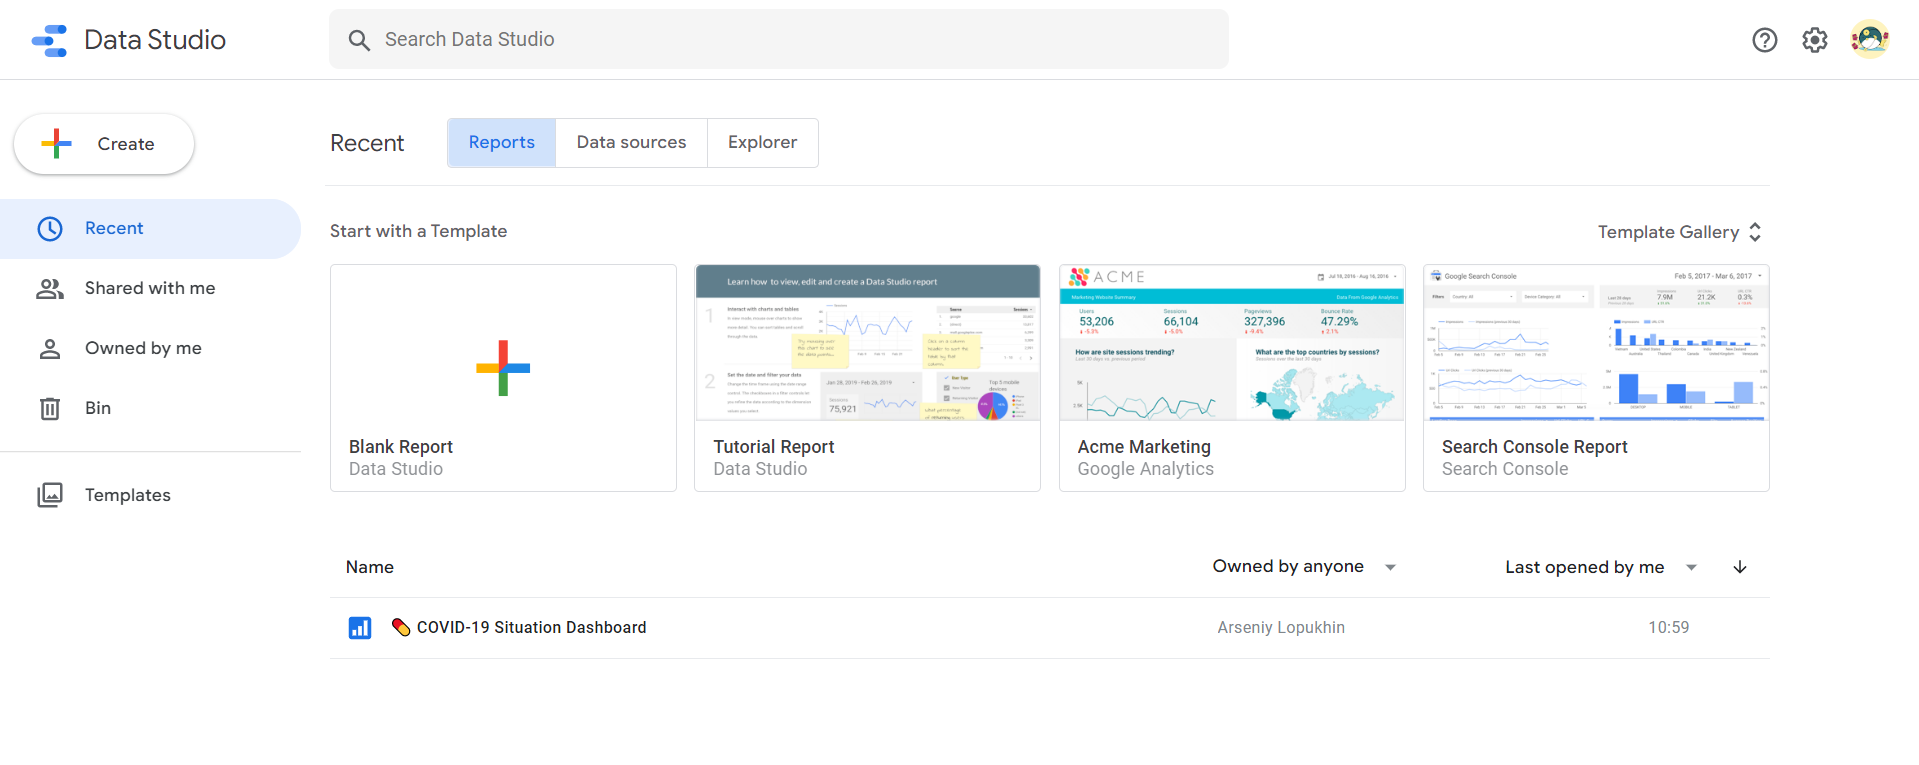
\includegraphics[width=12cm]{images/google_data_studio.png}
    \centering
    \caption{Google Data Studio ~\citep{google_data_studio}}
    \label{fig:google_data_studio}
\end{figure}

Nebst unterschiedlichen Visualisierungen wie Linien-und Balkendiagrammen können auch verschiedene Datenquellen über sogenannte ``Connectors`` angebunden werden (siehe Abbildung \ref{fig:google_data_studio_connectors}).

\begin{figure}[h]
    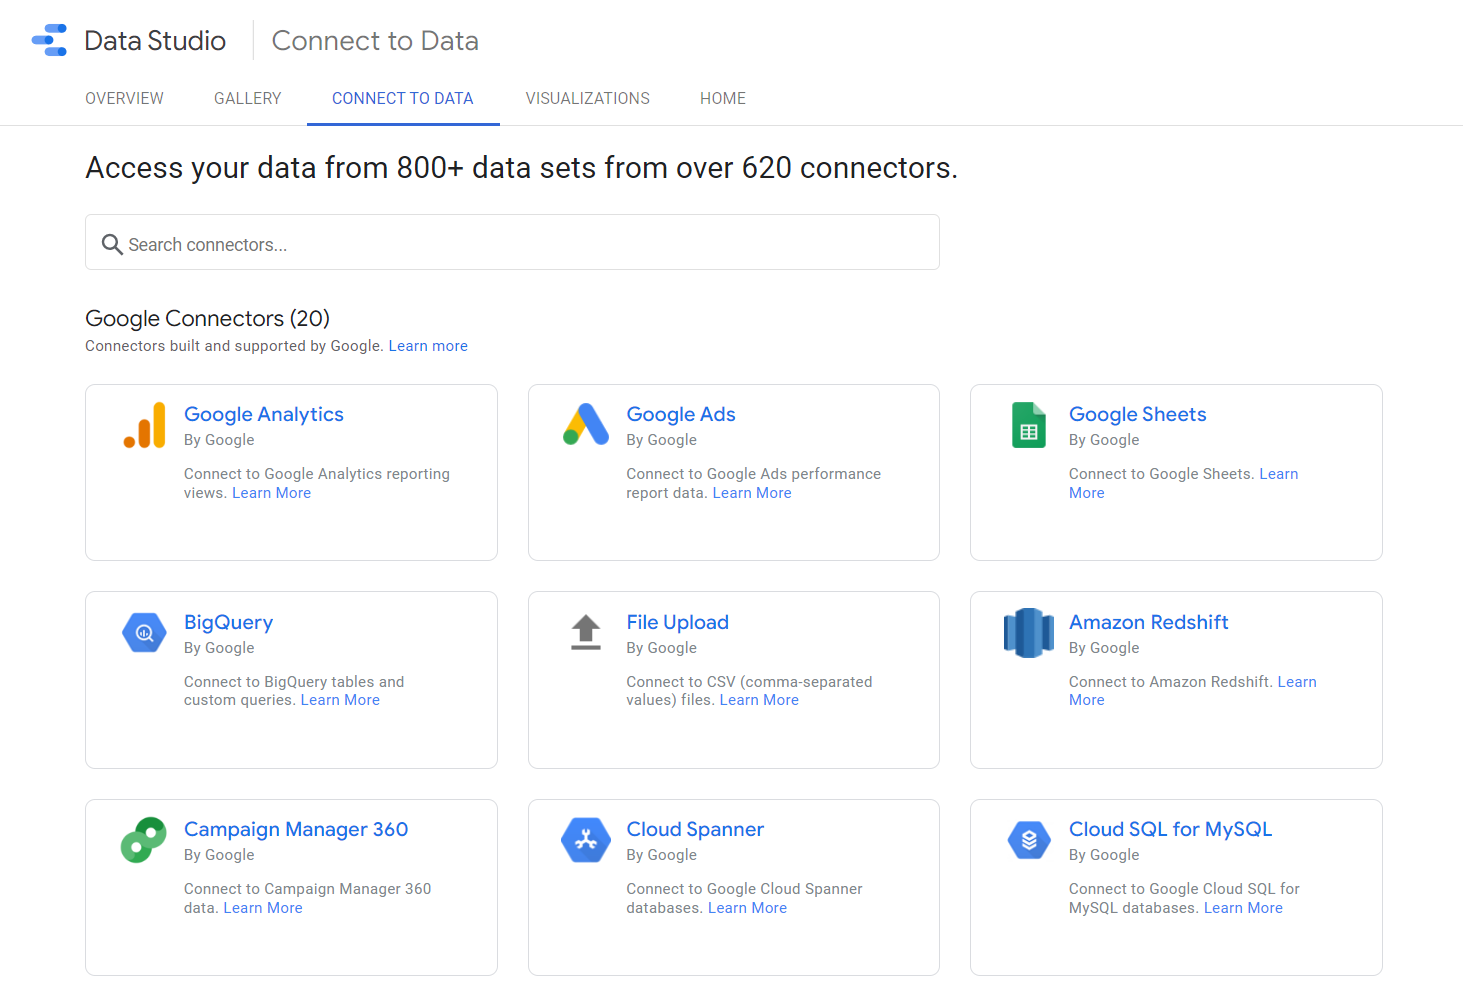
\includegraphics[width=12cm]{images/google_data_studio_connectors.png}
    \centering
    \caption{Google Data Studio Connectors ~\citep{google_data_studio_connectors}}
    \label{fig:google_data_studio_connectors}
\end{figure}

\clearpage
Gemäss der Studio von Barbazza setzte zum Beispiel Belgien Google Data Studio für die Erstellung eines interaktiven Corona Dashboards ein (siehe Abbildung \ref{fig:google_data_studio_corona_dashboard}).

\begin{figure}[h]
    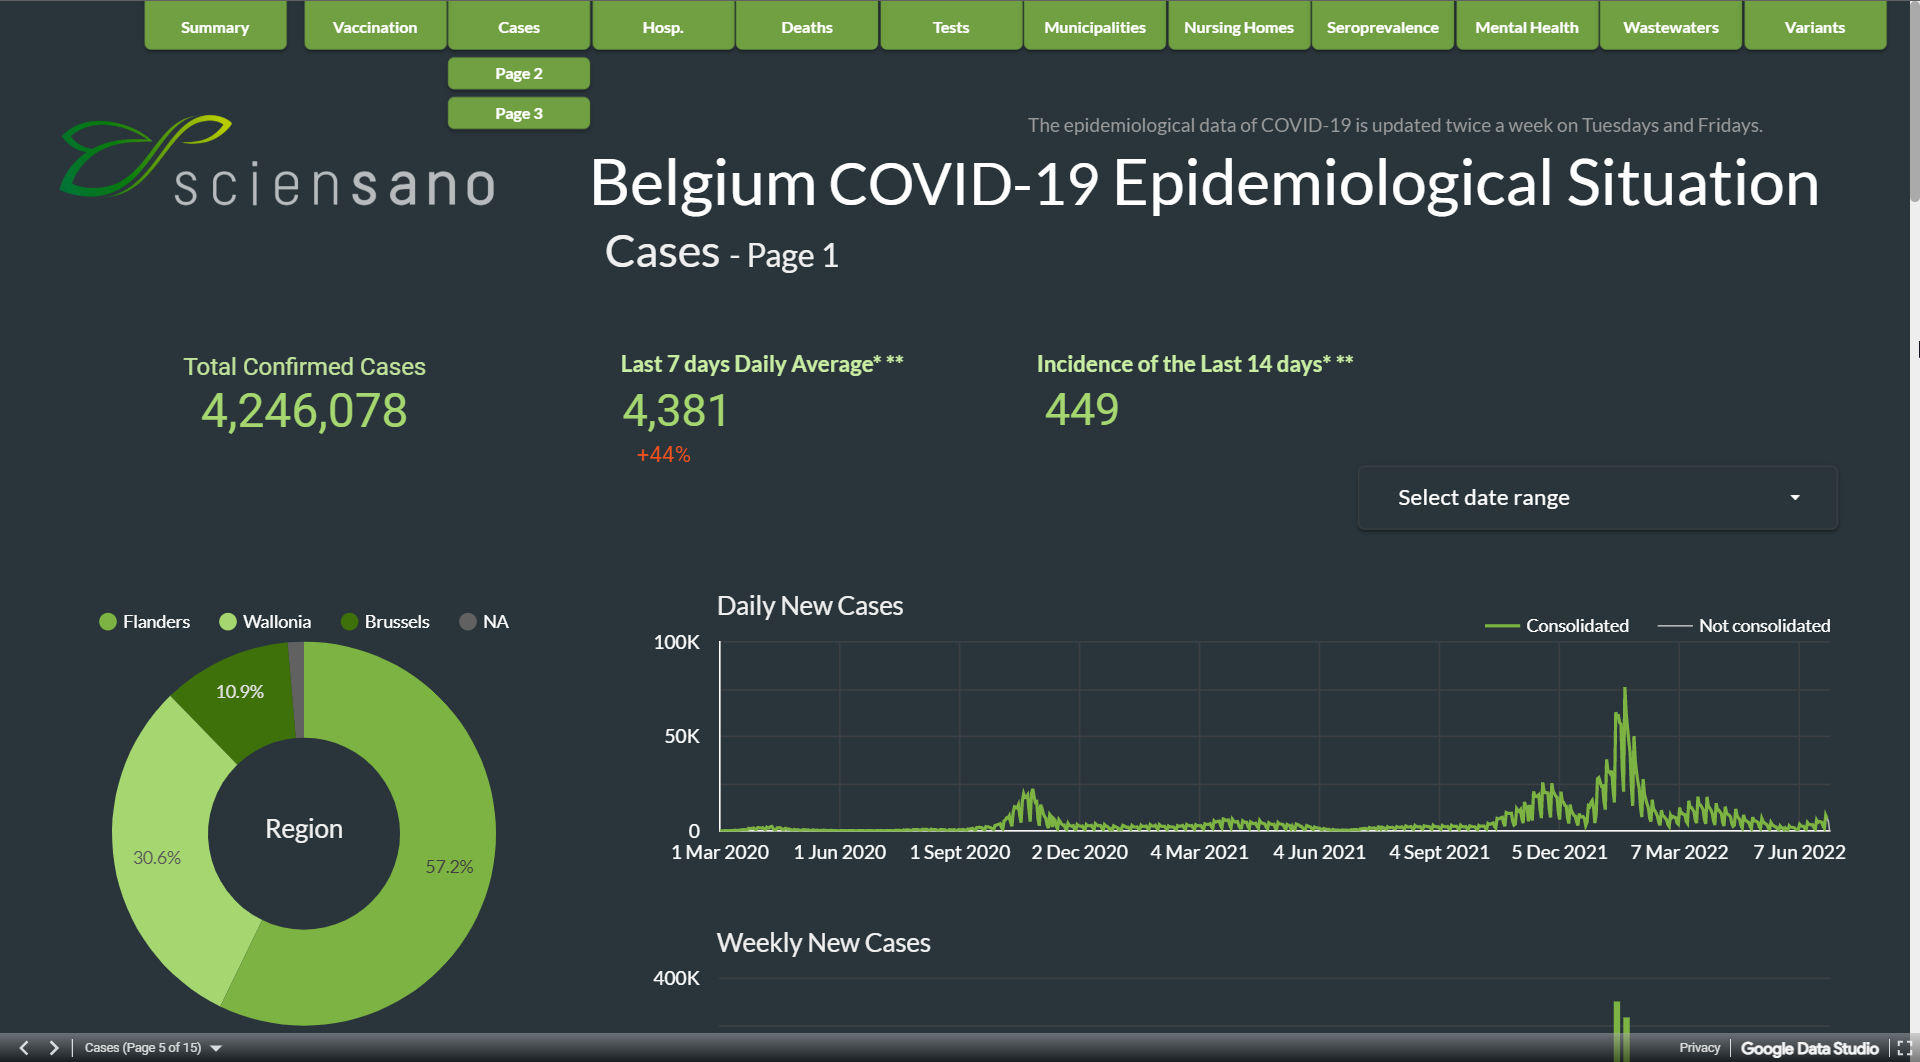
\includegraphics[width=12cm]{images/google_data_studio_covid_dashboard.png}
    \centering
    \caption{Corona Dashboard von Belgien welches mit Google Data Studio erstellt worden ist ~\citep{google_data_studio_corona_dashboard}}
    \label{fig:google_data_studio_corona_dashboard}
\end{figure}

\noindent
\textbf{Tableau}
\newline
\indent
Gemäss Sigdel zählt Tableau zu den Marktführern im Bereich der Daten Visualisierungen und Business Intelligence (Marktanteil 17\%) ~\citep{arcgis_comparison}. Im Vergleich zu ArcGIS ist der Preis von Tableau ebenfalls kostengünstiger. Tableau weisst seine Stärken vorallem bei nicht geografischen Daten auf. Hier bietet Tableau viele unterschiedliche Datenvisualisierungen und leichte Anpassungsmöglichkeiten ~\citep{arcgis_comparison}.

Ein Corona Dashboard, welches mit der Tableau Software realisiert wurde, ist das Dashboard von Estonia (siehe Abbildung \ref{fig:tableau_dashboard}).

\begin{figure}[h]
    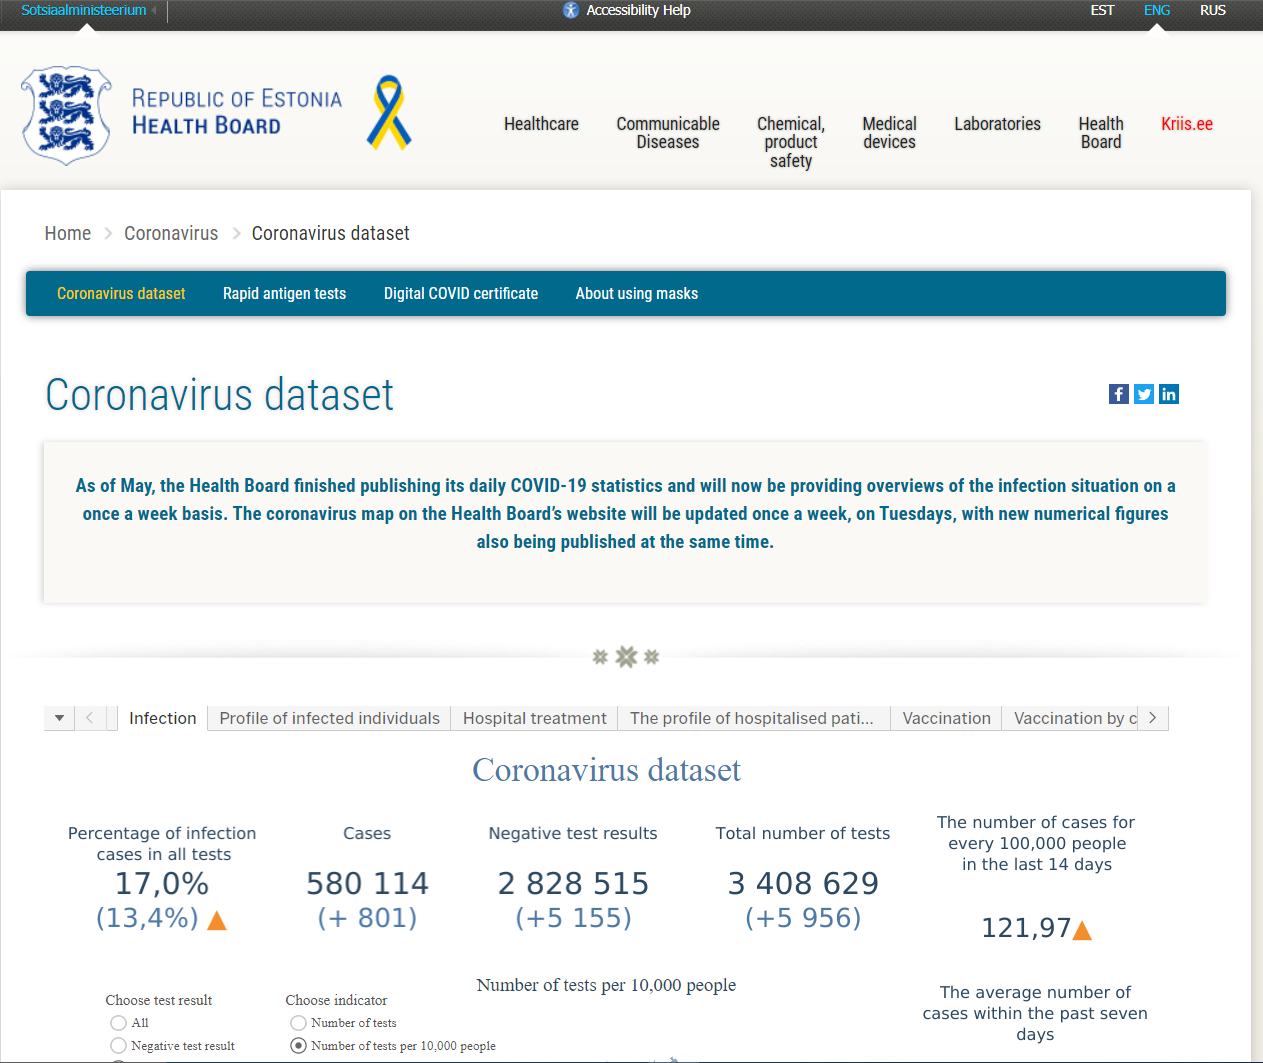
\includegraphics[width=10cm]{images/tableau_dashboard.png}
    \centering
    \caption{Corona Dashboard von Estonia welches mit Tableau erstellt wurde ~\citep{tableau_dashboard}}
    \label{fig:tableau_dashboard}
\end{figure}

Kommerzielle Lösungen wie Tableau und ArcGIS bieten viele Möglichkeiten um Dashboards zu gestalten und unterschiedliche Datenquellen anzubinden. Jedoch haben diese Lösungen unterschiedliche Expertisengebiete, welche je nach Anwendungsfall zu berücksichtigen sind. Tableau sowie ArcGIS sind nicht frei erhältlich, bieten aber professionellen Support bei Problemen an. Dem gegenüber stehen kostenfreie Lösungen wie Google Data Dashboard. Jedoch existiert bei solchen Lösungen nicht die gleiche Supportqualität. Alle Lösungen bieten ein Vorlagensystem für die Erstellung von Dashboards an. Jedoch hat sich gemäss Barbazza gezeigt, dass kommerzielle Lösungen zu Beginn eine schnelle Entwicklungsphase von Dashboards ermöglichen, jedoch im späteren Verlauf durch inflexible Anpassungsmöglichkeiten und fehlende Mehrsprachigkeit ihren Wert mindern. Ein weitere ausschlagekräftiges Kriterium bei kommerziellen Lösungen ist die Datenspeicherung. Hier gilt es zu beachten wo genau die Daten gespeichert werden und ob die entsprechenden Datenschutzrichtlinien eingehalten werden ~\citep[S. 9]{barbazza}.

\subsubsection{In-House Lösungen} \label{ch:theory_in_house_solutions}
In-House Lösungen sind selbst entwickelte Lösungen. Der Vorteil von diesen Lösungen besteht darin, dass volle Kontrolle über die Funktionalitäten der Software besteht. Jedoch sind In-House Lösungen mit hohen Entwicklungs- und Wartungskosten verbunden. Im Rahmen dieser Arbeit wird der Fokus bei den In-House Lösungen \textbf {auf Web Technologien gelegt}. Ein zentraler Vorteil von webbasierten Dashboards liegt darin, dass sehr einfach Visualisierungen von Echtzeitdaten möglich sind ~\citep[S. 34]{information_dashboard_design}. Ein weiterer ausschlaggebender Punkt ist die starke Verbreitung des Web Browsers, welcher auch auf jedem Smartphone verfügbar ist. Zudem können dank moderner Web Technologien anpassungsfähige Layouts mittels Responsive Design implementiert werden.

\clearpage
\noindent
\textbf{Technologien für die Erstellung von Frontend Web Applikationen}
\newline
\indent
Gemäss einer Umfrage von State of Javascript Survey 2020 sind die zwei populärsten Frontend Technologien zur Erstellung von Web Applikationen React sowie \textbf{Angular} (siehe Abbildung \ref{fig:most_used_frontend_frameworks}). Der Hauptfokus der Arbeit wird hierbei auf das Angular Framework gelegt.

\begin{figure}[h]
    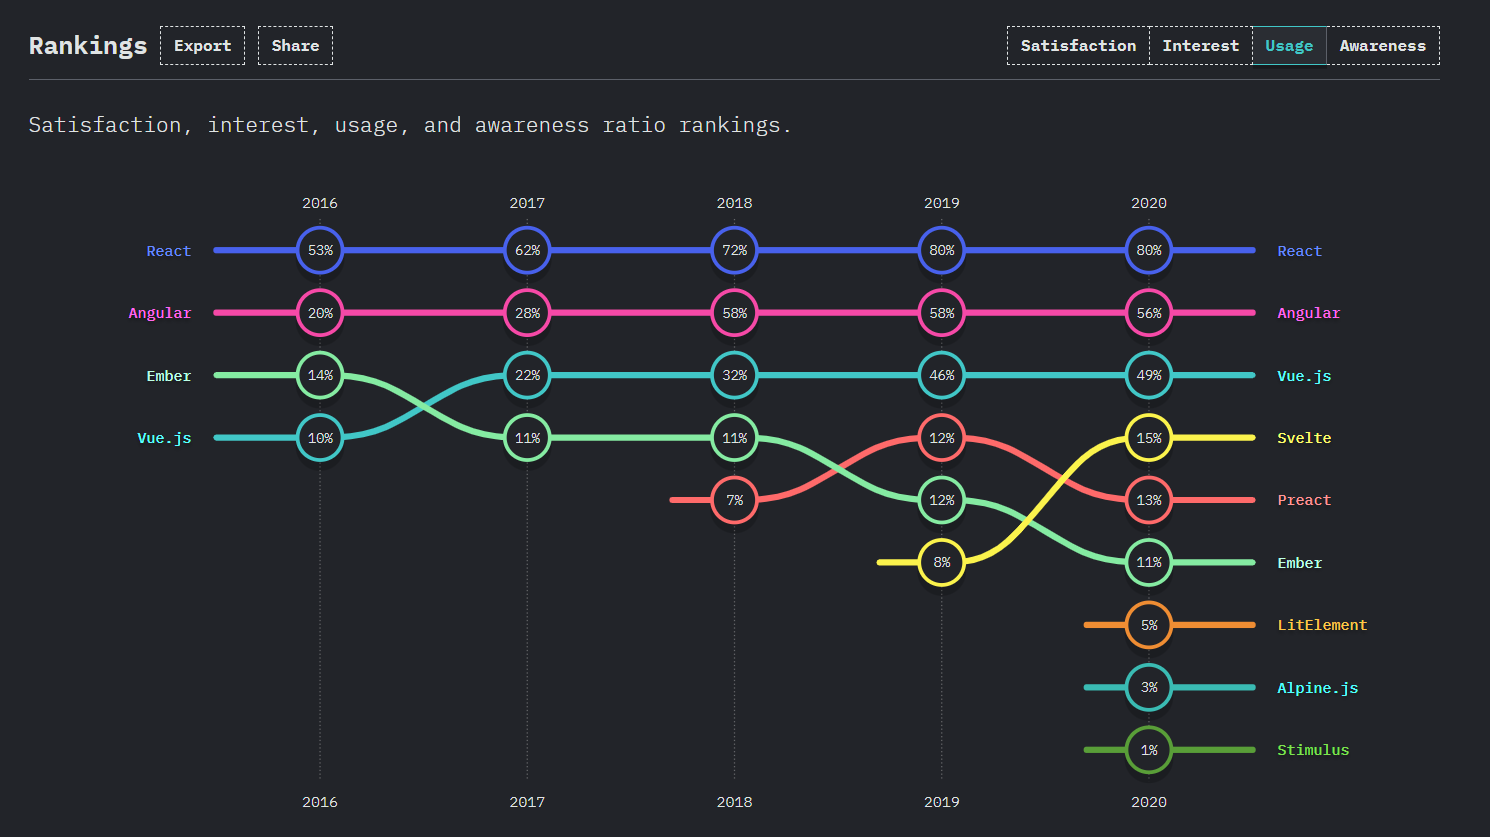
\includegraphics[width=12cm]{images/most_used_frontend_frameworks.png}
    \centering
    \caption{Meist verwendete Frontend Technologien zur Erstellung von Web Applikationen ~\citep{most_used_frontend_frameworks}}
    \label{fig:most_used_frontend_frameworks}
\end{figure}

\noindent
\textbf{Angular}
\newline
\indent
Angular ist ein Open Source Web Framework das auf einem \textit{Komponenten basierten Ansatz} aufgebaut ist und von der Firma Google sowie freiwilligen Personen entwickelt wird ~\citep{what_is_angular}. Open Source bedeutet, dass der Quellcode für jedermann frei verfügbar ist. Unter einer Komponente ist ein in sich abgeschlossenes Element zu verstehen, welches sowohl die visuellen Aspekte als auch die logischen Aspekte miteinander vereint. Die visuellen Aspekte werden dabei mithilfe der Technologien \gls{html} sowie \gls{css} umgesetzt werden. Die Logik der Komponente selbst wird hierbei in der Open Source Programmiersprache TypeScript, welche von Microsoft entwickelt wird, umgesetzt. TypeScript hat im Gegensatz zu JavaScript den Vorteil von \textit{statischer Typisierung}, d.h der Datentyp der Variablen wird explizit deklariert ~\citep{typescript}. Statische Typisierung hat den Vorteil, dass der Compiler (Programm welches den Code verarbeitet) Optimierungen vornehmen kann und bereits Fehlerquellen zur Kompilierungszeit anstelle der Ausführungszeit (wenn die Web Applikation bereits läuft) erkennt. Da der Komponenten basierte Ansatz ein zentrales Element des Angular Frameworks bildet, wird dieser nachfolgend mithilfe eines Beispiels illustriert. Die nachfolgenden Bilder wurden mithilfe der Website Carbon\footnote{https://carbon.now.sh/} erstellt.

\clearpage
\noindent
\textit{Implementierung der Komponentenlogik in TypeScript}
\newline
\indent
Eine Komponente beginnt mit der Deklaration von Metainformationen. Diese Metainformationen umfassen den Namen des Selektors, den Pfad zur \gls{html} sowie zur \gls{css} Datei der Komponente. Der Selektor bestimmt wie die Komponente bei der eigentlichen Verwendung zu bennenen ist. Anschliessend folgt die eigentliche Implementierung der Komponente selbst. Die Komponente welche zur Veranschaulichungszwecken vom Autor dieser Arbeit erstellt wurde, ist ein einfacher Zähler. Folglich benötigt die Komponente eine Zählvariable (counter). Die Variable ist hierbei vom Typ number (statische Typisierung), was einer Zahl entspricht. Mithilfe dieser Information weiss der Compiler, dass nur gewisse Aktionen wie Addition, Multiplikation etc. auf diesen Datentyp angewendet werden können. Somit sind bereits im Vorfeld Fehler vermeidbar, welche durch die Verwendung einer dynamischen Typisierung wie sie JavaScript mitbringt erst zur Laufzeit aufgefallen wären. Die Komponente bietet zudem noch eine Funktion zur Inkrementierung sowie Dekrementierung des Zahlenwerts an. Abbildung \ref{fig:angular_component_ts} veranschaulicht nocheinmals alle besprochenen Punkte auf einen Blick.

\begin{figure}[h]
    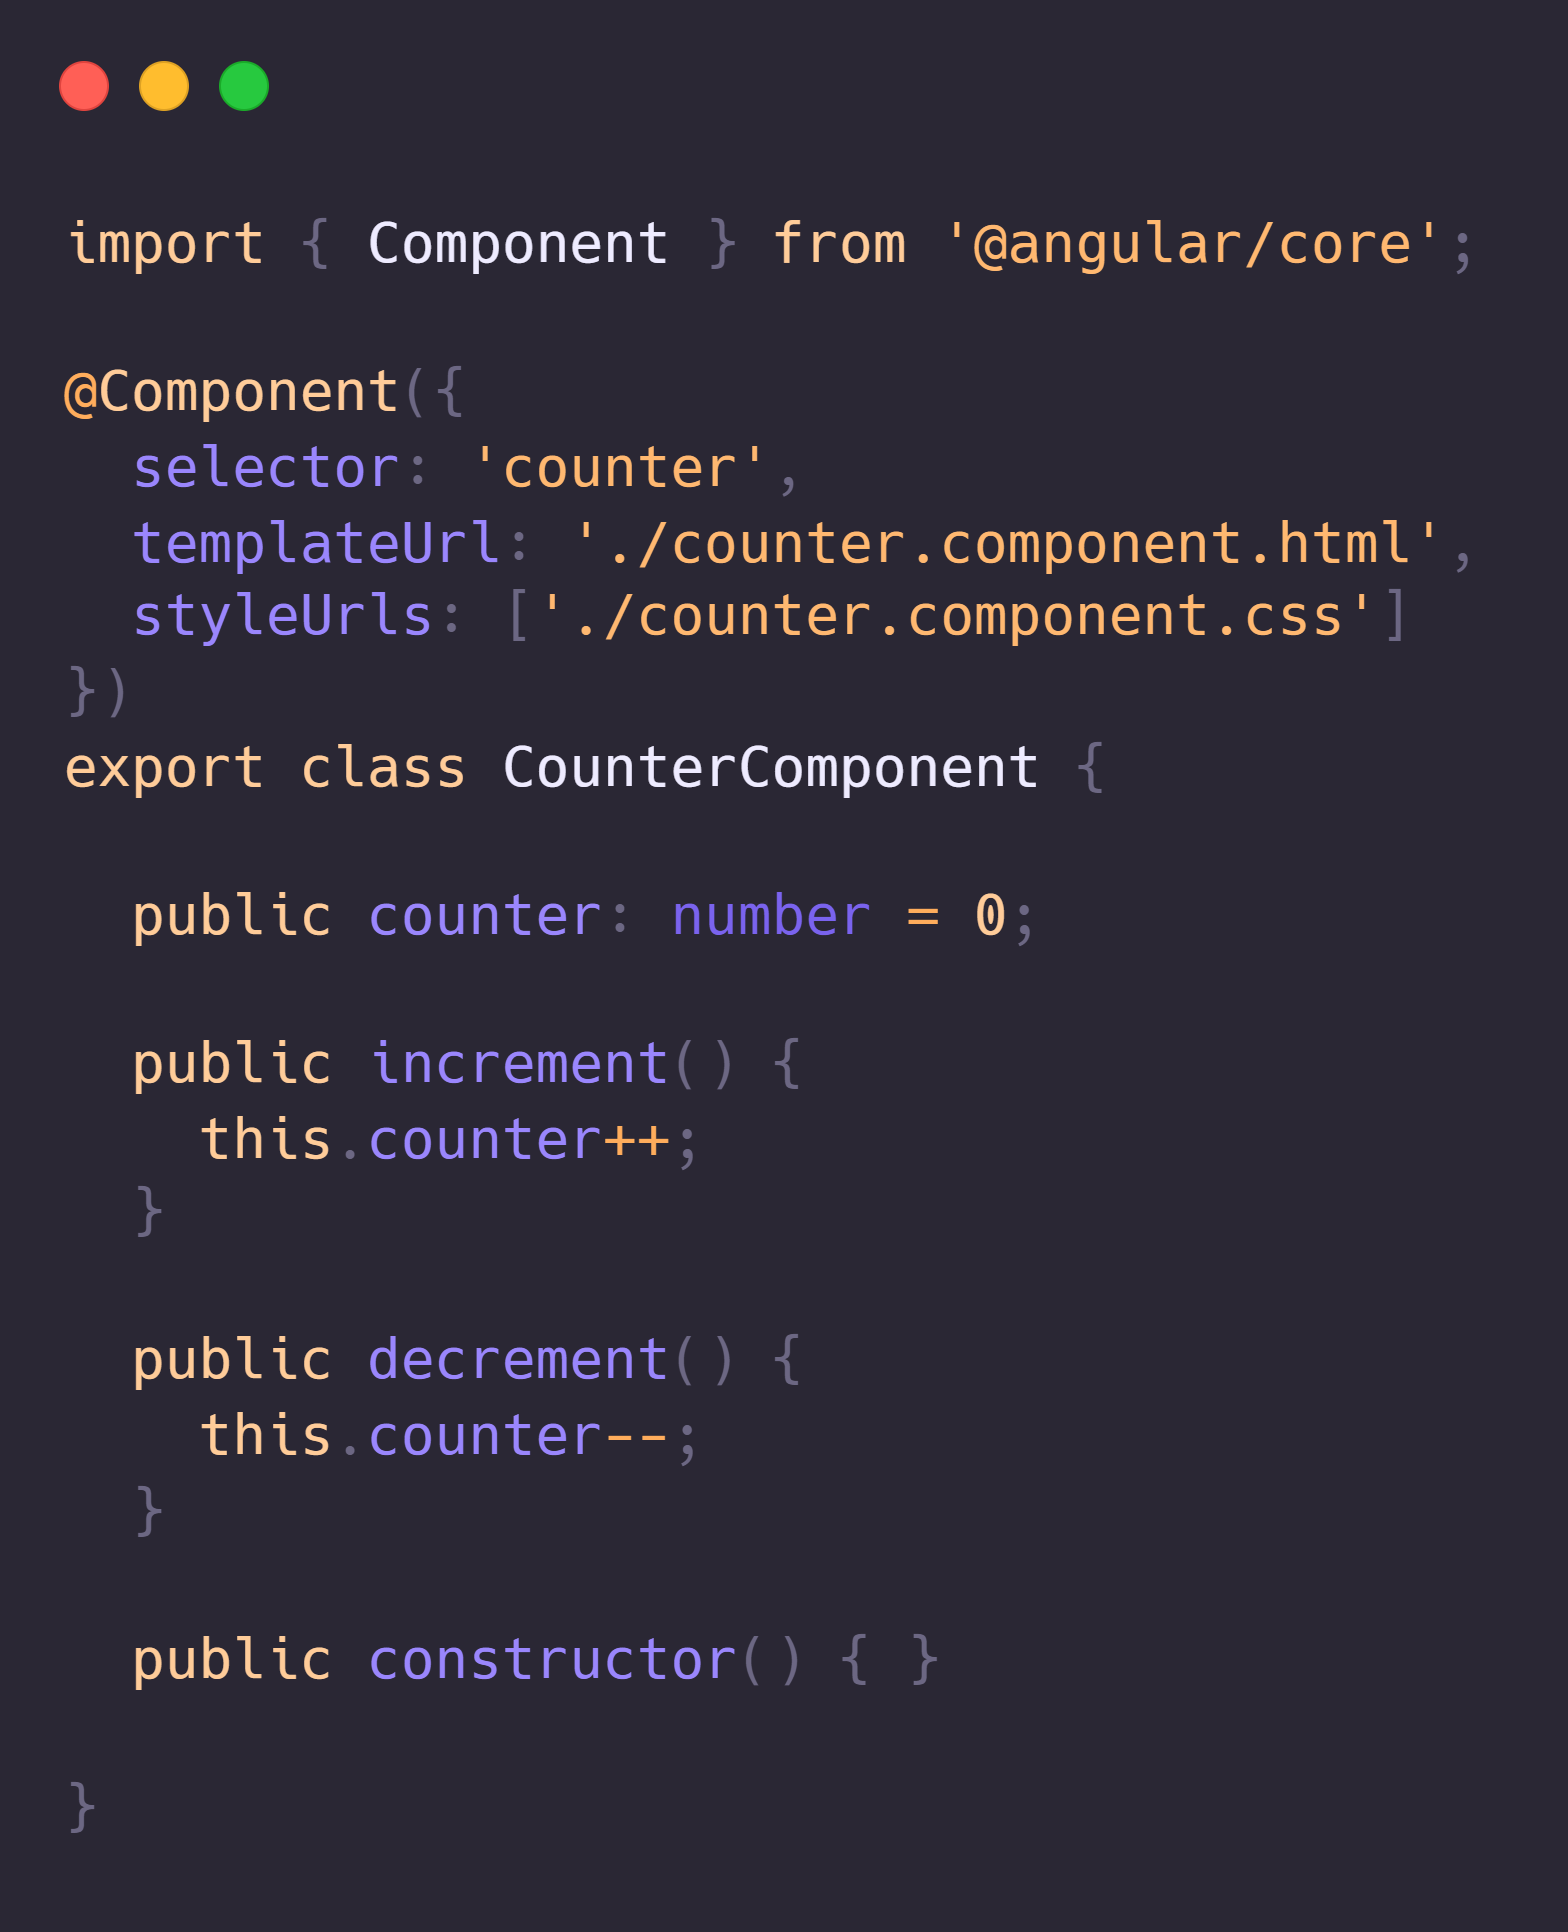
\includegraphics[width=10cm]{images/angular_component_ts.png}
    \centering
    \caption{Beispiel einer einfachen Angular Komponente (Komponentenlogik in TypeScript) (Eigene Darstellung)}
    \label{fig:angular_component_ts}
\end{figure}

\clearpage
\noindent
\textit{Implementierung der visuellen Gestaltung der Komponente in HTML}
\newline
\indent
Nebst der Logik der Komponente findet die visuelle Gestaltung in der verwiesenen \gls{html} sowie \gls{css} Datei statt (siehe templateUrl sowie styleUrls in Abbildung \ref{fig:angular_component_ts}). Der Zahlenwert wird hierbei in einem einfachen Paragraph Element dargestellt. Die Schreibweise mit den doppelten geschwungenen Klammern stellt sicher, dass wenn sich der Zahlenwert (counter Variable) aktualisiert, dies automatisch im \gls{html} ebenfalls reflektiert wird. Nebst der Darstellung des Zahlenwertes gibt es noch zwei Buttons welche an die Inkrementierungs sowie Dekrementierungs Funktionen gebunden sind. Abbildung \ref{fig:angular_component_html} veranschaulicht die oben aufgeführten Punkte noch einmal als Gesamtbild.

\begin{figure}[h]
    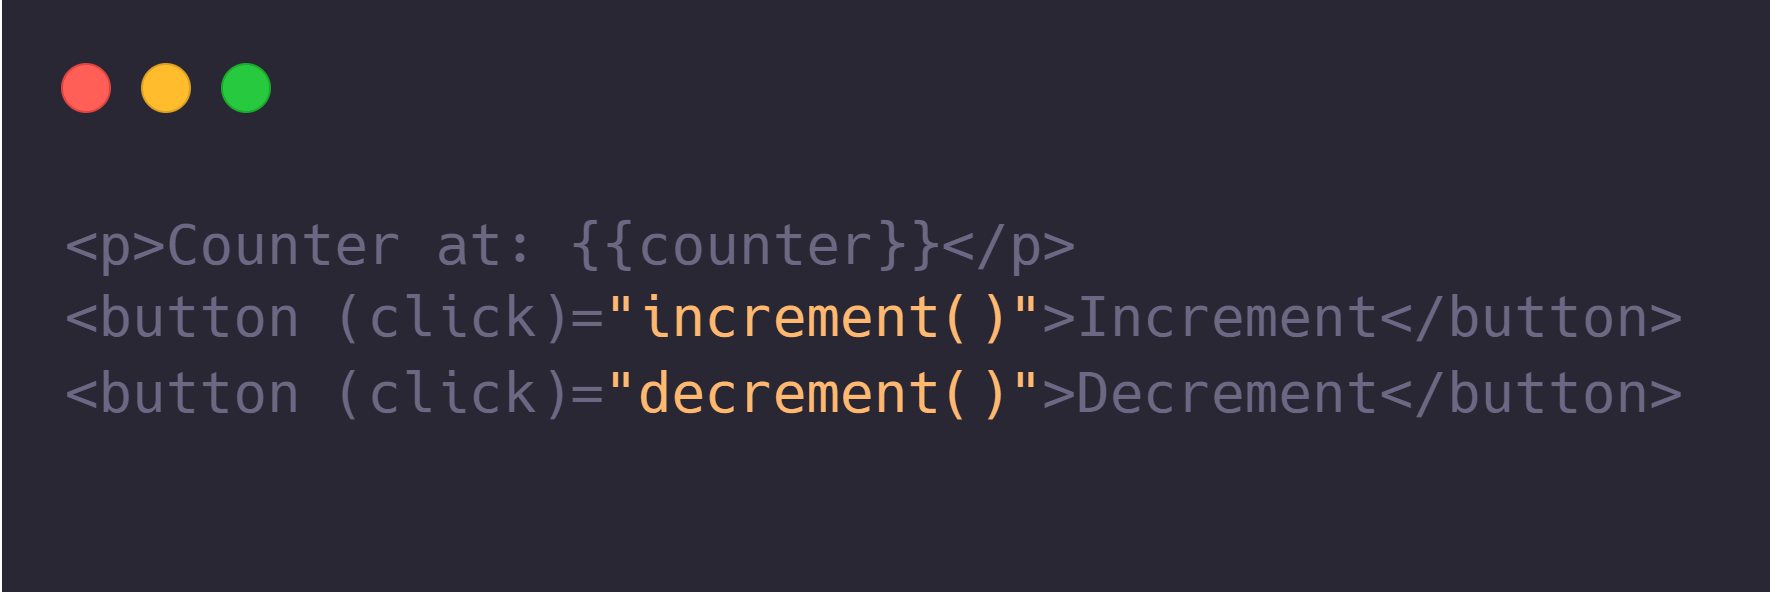
\includegraphics[width=12cm]{images/angular_component_html.png}
    \centering
    \caption{Beispiel einer einfachen Angular Komponente (visuelle Gesaltung in HTML) (Eigene Darstellung)}
    \label{fig:angular_component_html}
\end{figure}

\noindent
\textit{Verwendung der erstellten Komponente}
\newline
\indent
Die erstellte Komponenten muss nun in einem letzten Schritt noch verwendet werden. Dies ist einfach über die Verwendung des definierten Selektors (siehe selector in  Abbildung \ref{fig:angular_component_ts}) möglich (siehe Abbildung \ref{fig:angular_component_usage}). Die eigentliche Visualisierung im Browser kann der Abbildung \ref{fig:angular_component_browser} entnommen werden.

\begin{figure}[h]
    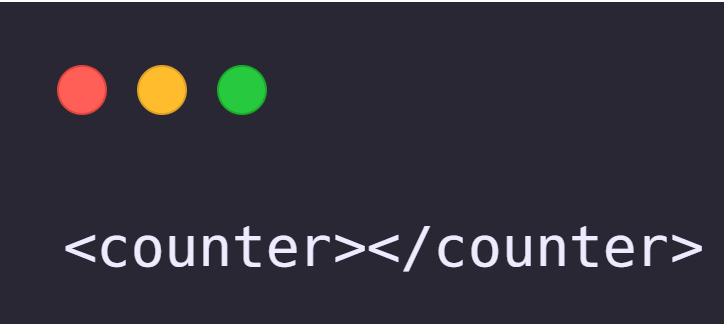
\includegraphics[width=6cm]{images/angular_component_usage.png}
    \centering
    \caption{Verwendung der erstellten Angular Komponente (Eigene Darstellung)}
    \label{fig:angular_component_usage}
\end{figure}

\begin{figure}[h]
    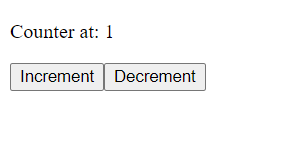
\includegraphics[width=6cm]{images/angular_component_browser.png}
    \centering
    \caption{Darstellung der Angular Komponente im Browser (Eigene Darstellung)}
    \label{fig:angular_component_browser}
\end{figure}

\noindent
\textit{CLI Tools}
\newline
\indent
Das Erstellen von Komponenten sowie das Erzeugen der notwendigen \gls{html} und \gls{css} Dateien bietet Raum für Automatisierung. Angular bietet aus diesem Grund \gls{cli} Tools an. Mithilfe der \gls{cli} Tools können sowohl das Generieren von Angular Applikationen sowie das automatische Erstellen von Komponenten etc. automatisiert werden. Ebenfalls können für den Produktionsbetrieb optimierte Dateien erstellt werden. Die hierfür notwendigen Befehle können einfach über ein Terminal eingegeben werden. Tabelle \ref{table:tbl:angular_cli_commands} veranschaulicht die wichtigsten Befehle in Bezug auf die oben erwähnten Punkte.

% Begin Angular CLI Table
\begin{table}[h]
\centering
\resizebox{\textwidth}{!}{%
\begin{tabular}{@{}ll@{}}
\toprule
\textbf{CLI Befehl} & \textbf{Beschreibung} \\ \midrule
ng new \textless{}application\textgreater{} & Erstellt eine neue Angular Applikation mit dem Namen \textless{}application\textgreater{} \\ \midrule
ng generate component \textless{}component\_name\textgreater{} & Erstellt eine neue Komponente mit dem Namen \textless{}component\_name\textgreater{} \\ \midrule
ng build & Erstellt einen für das Produktivsystem optimierten Build (Minifizierung der Dateien etc.) \\ \midrule
ng serve & Startet einen lokalen Web Server für die Entwicklung.\\ \bottomrule
\end{tabular}%
}
\caption{Gebräuchliche Angular CLI Befehle ~\citep{angular_cli}}
\label{table:tbl:angular_cli_commands}
\end{table}
% End Angular CLI Table

\noindent
\textbf{Technologien für Frontend Datenvisualisierungen}
\newline
\indent
Angular bietet ein Grundgerüst um mithilfe von Komponenten eine solide Web Applikationen implementieren zu können. Im Kontext von Dashboards und vorallem Corona sind jedoch nebst den visuellen Aspekten auch die Unterstützung von unterschiedlichen Datenvisualisierungen von hoher Relevanz. Barbazza merkte in Ihrer Studie ebenfalls die Limitationen von kommerziellen Lösungen in Bezug auf die Auswahl und Vielfältigkeit der Datenvisualisierungen an ~\citep[S. 9]{barbazza}. Im Rahmen dieser Arbeit wird der Fokus bezüglich Datenvisualisierungen auf das \textbf{Highcharts Framework} gesetzt, welches von rund 80 der 100 grössten Firmen weltweit verwendet wird ~\citep{highcharts}.
\newline

\newpage
\noindent
\textbf{Highcharts}
\newline
\indent
Das Highcharts Framework bietet eine breite Unterstützung für die Web sowie Mobilen Platformen an. Programmiersprachen wie Python, .NET sowie Web Frameworks wie React und Angular werden ebenfalls unterstützt. Highcharts unterteilt seine breite Palette an Datenvisualisierungen in verschiedene Module ~\citep{highcharts} an. Die Modularisierung hat den Vorteil, dass nicht das gesamte Framework sondern nur die benötigten Teile davon geladen werden müssen. Zudem bietet Highcharts zur jeder Art von Datenvisualisierung eine Beispielapplikation an, welche aufzeigt, wie die Visualisierungen im Kontext einer Web Applikation verwendet werden sollen (siehe Abbildung \ref{fig:highcharts_demo}).

\begin{figure}[h]
    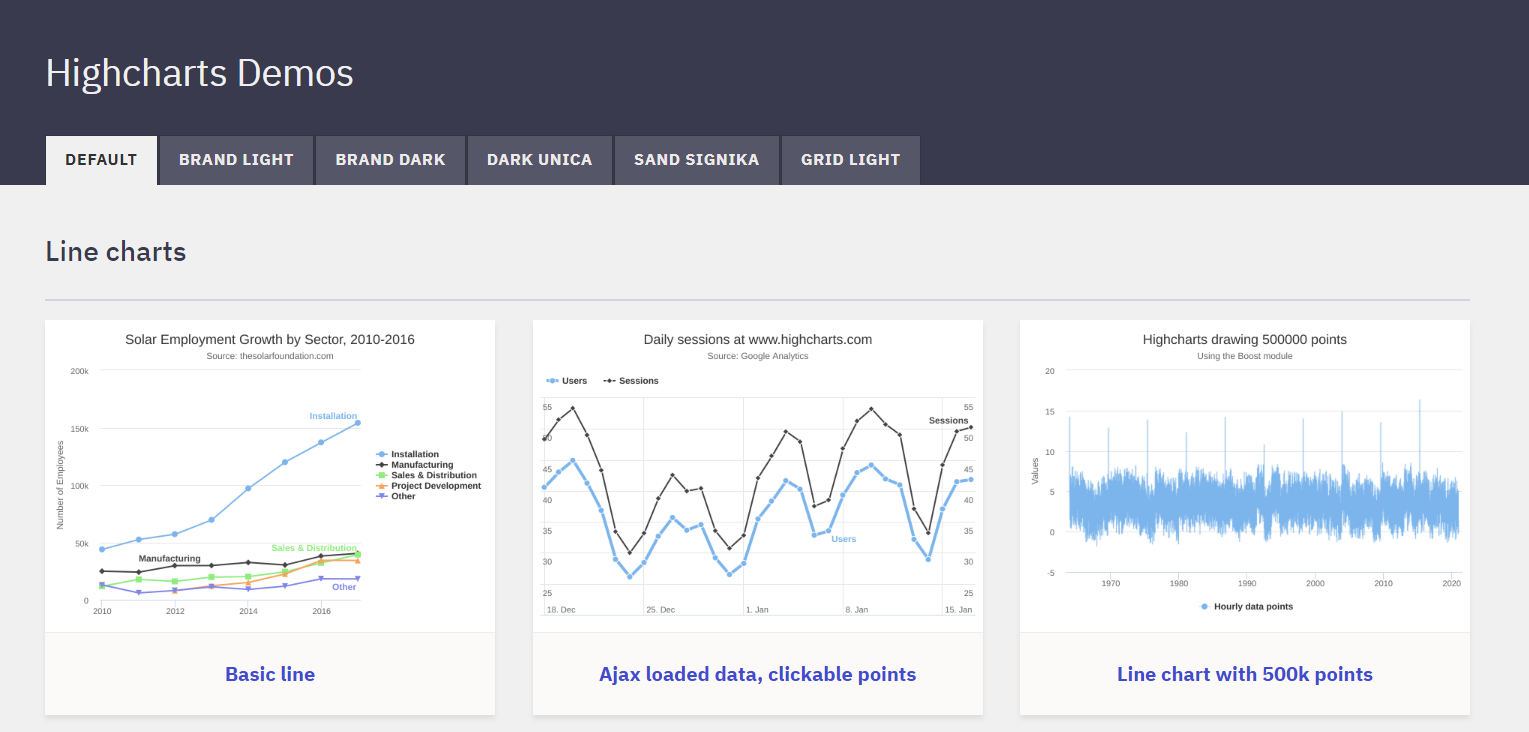
\includegraphics[width=12cm]{images/highcharts_demo.png}
    \centering
    \caption{Ausschnitt der Beispielapplikationen von Highcharts ~\citep{highcharts_demo}}
    \label{fig:highcharts_demo}
\end{figure}


 Ein Teil der verfügbaren Datenvisualisierungen kann der Tabelle \ref{table:highcharts_modules} entnommen werden. Die Tabelle wurde dabei basierend auf den verfügbaren Beispielapplikationen pro Modul erstellt.

% Begin Highcharts Modules
\begin{table}[h]
\centering
\resizebox{\textwidth}{!}{%
\begin{tabular}{@{}ll@{}}
\toprule
\textbf{Highcharts Modul} & \textbf{Datenvisualisierungen (Englischer Begriff)} \\ \midrule
Highcharts JS & Line charts, Area charts, Column and bar charts, Pie charts, Scatter and bubble charts, Combinations \\ \midrule
Highcharts Stock & Area charts, Depth charts, Column, Column Range \\ \midrule
Highcharts Maps & Heat Map, Bubble Map, Tile map, Spider map, Honeycomb \\ \midrule
Highcharts Gantt & Gantt chart \\ \bottomrule
\end{tabular}%
}
\caption{Ausschnitt der verfügbaren Visualisierungsarten pro Highcharts Modul (Eigene Darstellung)}
\label{table:highcharts_modules}
\end{table}
% End Highcharts Modules

Nebst dem modularen Aufbau ist Highcharts zudem sehr performant und kann ohne Probleme Millionen von Datenpunkten in weniger als einer Sekunde darstellen ~\citep{highcharts_fast_rendering}. Des Weiteren kann Highcharts im Rahmen von \textbf{nicht kommerziellen Projekte} ohne irgendwelche finanziellen Kosten eingesetzt werden ~\citep{highcharts_free}.